%%**************************************************************
%% GIS project report
%%**************************************************************

% possible structure
% x Estimation of the solar Potential with 3D CityDB (Introduction) DONE
% x.2 Workflow (Steffen) DONE
% x.3 Basics of PV systems (Hannah)DONE
% x.4 Basics of ST systems (Steffen) DONE
% x.5 Solar irradiance (Hannah) DONE
% 	x.5.1 Tilt (Hannah) DONE
% 	x.5.2 azimuth (Hannah) DONE
% 	x.5.3 satel light db (Hannah) DONE
% x.6 Roof surface area DONE
% 	x.6.1 simple reduction (Steffen) DONE
% 	x.6.2 reduction due to building age classes (Steffen) DONE
% x.7 Shadowing (Steffen) DONE
% x.8 Calculation of the potential DONE
%	x.8.1 Photovoltaic (Hannah) DONE
% 	x.8.2 Solar Thermal (Steffen) DONE
% x.9 Results (Steffen)
%	x.9.1 Test Area (Steffen)
% 	x.9.2 Validation (Steffen)
% x.10 Visualization (Hannah)
% x.11 Conclusion (Hannah) First version is DONE
% x.12 Future Work (Hannah) DONE


%\documentclass[10pt,a4paper,portrait]{article}
\usepackage{geometry}                % See geometry.pdf to learn the layout options. There are lots.
\geometry{a4paper}                   % ... or a4paper or a5paper or ... 
%\geometry{landscape}                % Activate for for rotated page geometry
\usepackage[parfill]{parskip}    % Activate to begin paragraphs with an empty line rather than an indent
\usepackage{graphicx}
\usepackage{subfig}
\usepackage{amssymb}
\usepackage{amsmath}
\usepackage{epstopdf}
\usepackage{multicol}
\usepackage{amsmath}
\usepackage{listings}
\usepackage{url}
\usepackage{multirow}
\usepackage{color}
\definecolor{grey}{rgb}{0.5,0.5,0.5}
\definecolor{darkgreen}{rgb}{0.5,0.5,0.0}
\lstset{ %
language=Matlab, % the language of the code
basicstyle=\ttfamily, % the size of the fonts
       % that are used for the code
numbers=left, % where to put the line-numbers
numberstyle=\footnotesize, % the size of the
        %fonts that are used for the line-numbers
stepnumber=1, % the step between two
       % line-numbers. If it's 1, each line 
keywordstyle=\color{darkgreen}, % Keywords
       % font ('*' = uppercase)
commentstyle=\color{grey},
numbersep=5pt, % how far the line-numbers are
       % from the code
backgroundcolor=\color{white}, % choose the
        %background color. You must add \usepackage{color}
showspaces=false, % show spaces adding
        %particular underscores
showstringspaces=false, % underline spaces
        %within strings
showtabs=false, % show tabs within strings
       % adding particular underscores
frame=single, % adds a frame around the code
tabsize=2, % sets default tabsize to 2 spaces
captionpos=b, % sets the caption-position to
        %bottom
breaklines=true, % sets automatic line
        %breaking
breakatwhitespace=false, % sets if automatic
        %breaks should only happen at whitespace
 % show the filename of files included with
       % \lstinputlisting;
 % also try caption instead of title
escapeinside={\%*}{*)} % if you want to add a
       % comment within your code
}
\DeclareGraphicsRule{.tif}{png}{.png}{`convert #1 `dirname #1`/`basename #1 .tif`.png}
% 
% \begin{document}
% 
% % Titlepage with task representation
% \input{include/title}	
% \newpage
% 	

% Introduction + workflow
-This chapter will describe how the system will be designed, how the Field of application can be modelled, what functionalities can be planned-

\section{Einsatzgebiet}
Um präzise beschreiben zu können was das System tun können muss, ist es notwendig vorher konkret die vorliegende Situation oder das existierende Problem zu definieren. Solche eine Definition sollte eine Beschreibung der Umgebung beinhalten in der das System eingesetzt werden soll. Nimmt man eine Modellierungssprache zur Hilfe, um die Umgebung zu beschrieben, ist es später einfacher daraus Rückschlüsse auf mögliche Probleme zu ziehen. Für ein solches Modell müssen die Fragen beantwortet werden, in welche Objekte sich die Umgebung aufgliedert, wie diese interagieren und welche Funktionalitäten diese dafür verwenden.Aber auch die teilhabenden Akteure und ihre konkreten Anforderungen an das System müssen modelliert werden. Mit Hilfe von exemplarischen Anwendungsfällen werde ich beschreiben was der tatsächliche Bedarf des Nutzers ist, und wie dieser gedeckt werden kann.

Bevor ich mit dem technischen Ausformulieren der Modellierung beginne, möchte ich kurz in die Thematik einleiten: Das System welches ich mit dieser Arbeit konzeptioniere soll Feldingenieuren helfen im Feld mit den Messungen und Daten verschiedener Sensoren zu arbeiten. Als konkretes Beispiel werde ich den Einsatz des Systems bei der Bauwerksüberwachung mithilfe eines Sensornetzwerkes beschreiben.

Die Überwachung von Bauwerken mittels eines Netzwerkes aus verschiedenen Sensoren hilft ihre Sicherheit ohne den Einsatz großer Bautechnischer Überprüfungen einschätzen zu können. Damit ist es möglich Bauwerke auch weit über ihre geplante Lebensdauer hinweg zu erhalten. Ohne den Einsatz solcher Sensor Netzwerke können die zuständigen Gutachter bei Ablauf der geplanten Lebensdauer nicht darauf vertrauen, dass das Gebäude auch weiterhin den kontinuierlichen Belastungen gewachsen ist, und somit werden entweder umfangreiche Sanierungen Nötig, oder Gebäude werde geschlossen. Die Überwachung basiert auf der Messung von Veränderungen von verschiedenen Parametern wie zum Beispiel der Position , der Temperatur oder Feuchtigkeit von Bauteile oder der Abweichungen von charakteristischen Bewegungsmustern von Bauteilen, gemessen durch Beschleunigungssensoren. Die Parameter werden sowohl punktuell  verteilt über das gesamt Bauwerk, als auch gesamtheitlich die Struktur des Bauwerkes miteinbeziehend erhoben, siehe auch \citep{worden_overview_2004} \citep{farrar_introduction_2007} \citep{boller_structural_2004}. Für die Messungen werden zum einen automatisch kontinuierlich messende Systeme eingesetzt, und zum anderen seltenere manuelle Messungen, deren Ergebnisse manuelle in das System eingegeben werden. 

Für das bessere Verständnis möchte ich hier ein Beispielfall beschreiben: Ein Brücke erreicht ihre letzten Jahre der Betriebserlaubnis. Danach müssen entweder die Verkehrssicherheit erneut umfangreich geprüft, und zahlreiche Verschleißteile, deren Zustand schlecht zu beurteilen ist, ersetzt werden, oder die Verkehrssicherheit muss auf andere Art überprüft werden. Zahlreiche Sensoren werden an den einzelnen wichtigen Gebäudeteilen eingerichtet, und überwachen nun automatisch über einen bestimmten Zeitraum deren Verhalten und Veränderungen. In periodischen Abständen werden automatisch Diagnosen erstellt, basierend auf der Analyse der Messwerte, der Überprüfung des Materialverschleißes und einiger anderer Einflussgrößen. Eine detailliertere Beschreibung der verwendeten Messungen, Zeitskalen und Analysemethoden werden in den nachfolgenden Kapiteln beschrieben.

In der Einleitung der Arbeit möchte ich mich am Verlauf der Erstellung eines Pflichtenheftes für die Softwareentwicklung orientieren , da so am besten modelliert werden kann wie der Bedarf des Nutzers gedeckt werden kann, siehe auch \citep{gregor_engels_vorlesung_2006}. Beginnen werde ich mit einer textuellen Beschreibung der Situation. Danach folgt eine Modellierung der Prozesse und der Akteure mit ihren jeweiligen Anwendungsfällen. Zum Abschluss werde ich dann die daraus abgeleiteten notwendigen Funktionalitäten des System beschreiben.


\subsection{Modell des Problembereichs}
Die Abbildung \ref{fig:model_domain} zeigt ein UML Diagramm (Unified Modeling Language) das die im folgenden beschrieben verschiedenen Objekte des Systems beinhaltet. Das Modell beschreibt die Beziehungen der einzelnen Objekte untereinander und modelliert keine Aktivitäten oder Funktionen.

Die Umgebung in der das System eingesetzt werden wird besteht aus fünf verschiedenen Arten von Objekten und deren Beziehungen untereinander. Zentrales Objekt ist der Daten Server, der als Knoten für die Kommunikation zwischen den einzelnen Kompartimente dient. Diese sind hauptsächlich die Sensoren selbst, die jedoch ohne einen Server, der als Steuerungseinheit für jeden Sensor dient, nicht selbständig messen können. Der Server kontrolliert die Sensoren indem er sie aktiviert und deaktiviert. Nichtsdestotrotz können Sensoren in einem separiertem eigenem Netzwerk organisiert sein, das dann wiederum als einzelner Sensor behandelt wird. Die Sensoren senden ihre gemessenen Daten entweder aktiv an den Server beziehungsweise über den Server an die dem Server angeschlossene Datenbank, oder der Server ruft die Daten aktiv ab, und speichert diese dann in der Datenbank.

\begin{figure}[H]
	\centering
 	 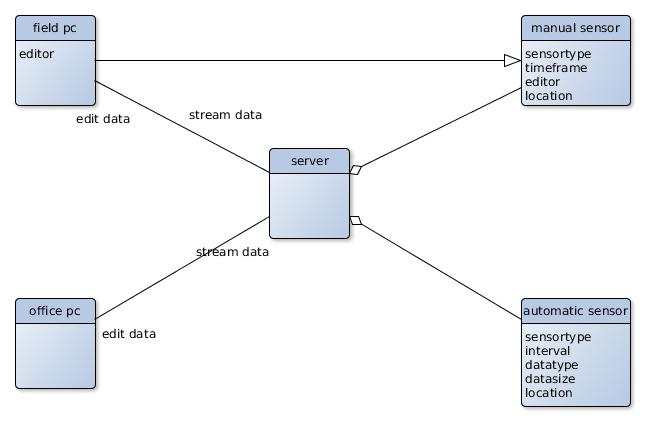
\includegraphics[scale=0.6]{graphics/model_of_issue.jpg} 
	\caption{Modell des Problembereiches mit relevanten Objekten, F. H. Euteneuer 2013}
	 \label{fig:model_domain}
\end{figure}

Die Datenbank die and den Server angeschlossen ist speichert sowohl Metadaten zu den Sensoren, als auch die gemessenen Werte. Unter Metadaten sind alle Informationen zu verstehen, die die Sensoren eindeutig beschreiben, und die für weitere Analysen der Messerwerte erforderlich sind (siehe auch im Glossar "Metadaten". Beispielsweise sind das die Positionen der Sensoren, die Messintervalle, die Sensortypen oder die übermittelten Datentypen.

Als Klient des Services kann im Prinzip jede Art von mobilen Systemen eingesetzt werden. Angeschlossen an die Datenbank dienen diese dann als bildgebender Teil des Systems. Da die Verknüpfung mit einem Server meist über das Protokoll TCP/IP geschieht, müssen mobile Geräte über eine Internetverbindung verfügen. Die Verwendung dieser Geräte bleibt dadurch begrenzt auf Gebiete innerhalb der Handynetz-Abdeckung. Für manuelle Messungen dient der mobile Klient zusätzlich als Eingabegerät für die Messwerte, sofern dies nicht über das Gerät selber erfolgen kann. Dadurch wird der mobile Klient in dem Modell sowohl als bildgebender Teil des Systems, als auch als Sensor behandelt, und ererbt damit die Eigenschaften des Sensor Objekts.

Das System will einen ganzheitlichen Ansatz verfolgen, und beinhaltet somit auch einen Teil der für die umfangreicheren Analysen zuständig ist, sowie durch eine Datenexportfunktion als Schnittstelle zu weiteren Algorithmen und System dient. Dieser Teil des System wird in dem Modell durch den "Desktop-Computer" repräsentiert. Die eigentliche Einrichtung und Planung des Systems wird erwartungsgemäß von diesem, dem bequemeren Arbeitsplatz (verglichen mit dem mobilen Klienten), durchgeführt werden. Zusätzlich zu den Eigenschaften des Feldcomputers sind somit erweiterte Verwaltungs- und Analysefunktionen als Eigenschaften dieses Objektes definiert.


\subsection{Geschäftsprozesse}
Wichtigste Entscheidungshilfe für die Nutzung solch eines Systems wird die Eigenschaft des Systems, eine entscheidungsunterstützende Funktion zu erfüllen, sein. Das System ist fokussiert auf die wichtigen Werkzeuge die die Arbeit des Feldingenieurs vereinfachen sollen, und lässt unwichtige oder komplizierte Werkzeuge komplett weg. Außerdem werden die Informationen die im Feld auf dem mobilen Klienten angezeigt werden derart reduziert, dass lediglich aussagekräftige Werte, die damit Entscheidungen unterstützen können, angezeigt werden. In dem vorherigem Kapitel habe ich den Problembereich beschrieben, nun möchte ich die verschiedenen Prozesse skizzieren die ein Nutzer durchführen könnte.

\begin{figure}[H]
	\centering
 	 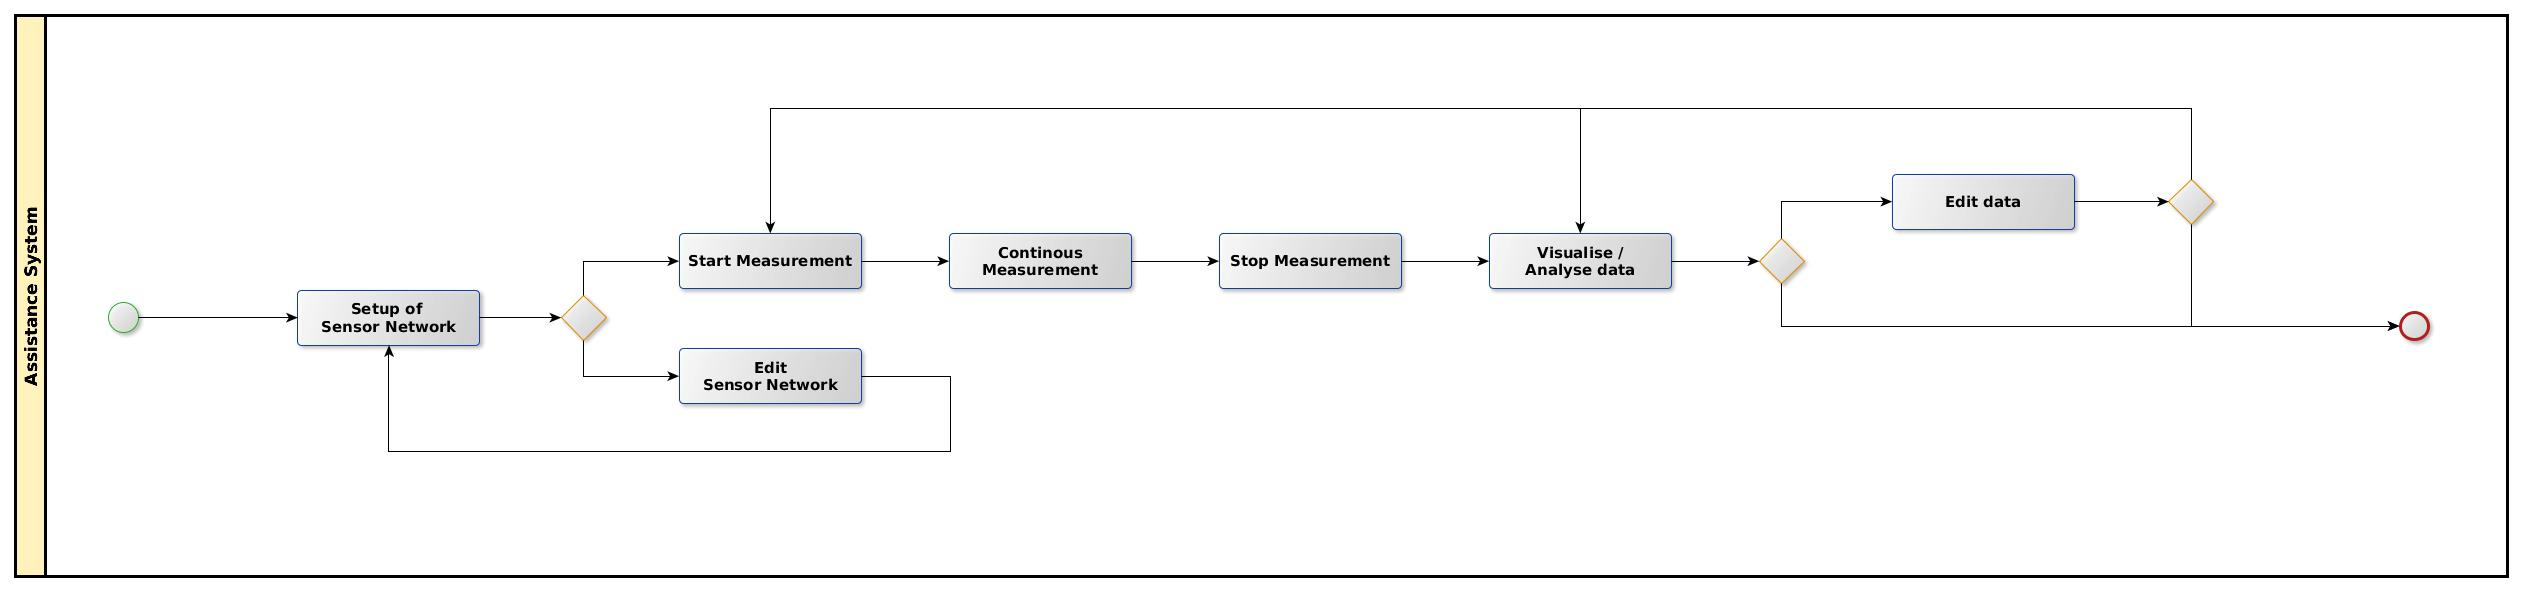
\includegraphics[scale=0.2]{graphics/bpmn_business-processes.jpg} 
	\caption{BPMN (Business Process Model and Notation) Modell relevanter Aktionen welche in dem System durchgeführt werden, F. H. Euteneuer 2013}
	 \label{fig:model_business-processes}
\end{figure}

Ich habe drei verschiedene Hauptaktionen identifiziert, die ein Nutzer durchführen könnte: Das manuelle Messen von Werten, das manuelle Editieren bereits gemessener Werte, und das automatische kontinuierliche Messen. Die Abbildung \ref{fig:model_business-processes} veranschaulicht mittels eines UML Activity Diagrams (UML Aktivitäten Diagramm) die einzelnen Abläufe dieser Aktionen.

Die manuelle Messung beginnt mir der normalen Messung der Werte. Im zweiten Schritt erfolgt die Eingabe der Werte in das System. Die Werte werden automatisch auf ihre Validität hin überprüft, und erste einfache statistische Analysen werden erstellt. Diese erste Statistik ist erforderlich um Informationen über die Qualität der Messung zu erhalten, und dem System die Möglichkeit zu bieten fehlerhafte Messungen zu bemängeln und Neumessungen vorzuschlagen.

Der Nutzer wird die Möglichkeit haben vergangene Messungen manuell zu bearbeiten. Dazu muss ein Datensatz (Üblicherweise ein Messwert) ausgewählt werden, und der Nutzer kann dann entscheiden ob die betreffende Messung wiederholt werden soll, oder die Werte manuell geändert werden sollen. Bei einer Wiederholung der Messung wird die Prozesskette der manuellen Messung durchlaufen.


The automatic measurements are the most important one for the described SHM. The will be the backbone of the system, nevertheless they are using similar functionalities. The user will initially be able to set the sensor network up. Which means to enter metadata about the used sensors like position, reference system, type of sensor, measurement interval, etc. A more detailed description of what is needed for such a setup will follow in the methodical part. After the setup, the user is able to start the measurements with the defined parameter, or the edit the settings.

As a conclusion of this chapter, I would like to point out that this list is only representing functionalities of a basic system, and should not be understood as being complete.


\section{Functionalities}
This chapter will describe what the system should provide to solve the problem and/or make the existing situation better: Which functionalities should be part of the system. To get closer to a possible solution, the different stakeholders and their use cases in the domain of structural health monitoring must be defined and described.

\begin{figure}[H]
	\centering
 	 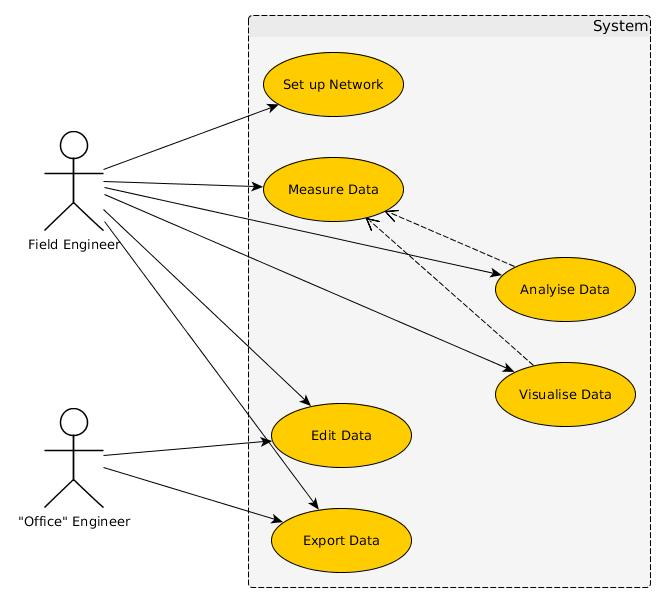
\includegraphics[scale=0.6]{graphics/uml_functionalities.jpg} 
	\caption{UML Use Case Diagram of the described System describing two different users and their use cases. By F. H. Euteneuer 2013}
	 \label{fig:model_functionalities}
\end{figure}

\subsection{Usergroups}
As a main source for information and parameter for the concept of a software, the usergroups are of large importance. I will analyse the involved usergroups and their needs respective expectations to get those information. As the figure \ref{fig:model_functionalities} is already representing, I have identified two main usergroups which might be involved in the processes.

\subsubsection{Field-engineer}
The group of field-engineers can described as the executive persons which are dealing with the direct measurements, observations and setup of an automatic measurement network. This group can be categorised by its technically limits, which are:
\begin{itemize}
\item the small screen-size of the mobile computers (quality of visualisation is limited)
\item the lack of input facilities (e.g. only digital keyboard on a handheld computer)
\item high weight of not handheld instruments (e.g. a conventional laptops too heavy for using while walking/standing)
\end{itemize}
But nevertheless, this usergroup has the most challenging requirements on the system when speaking about visualisation options or analysis computation in advance. It is the central target usergroup for this system, therefore it should fit mostly to its requirements.


\subsubsection{Office-engineer}
Usually the field-engineer and the office-engineer are combined in one person. One part of an observation project is dealing with the field-work, the setup, measurements and maintenance. And the other part is the precise analysis of the data, the post processing and its interpretation. Due to a high quality equipment in the offices, this part is mostly better solvable for a software. Here does not the system has to be restricted by the environment, but the system is making its demands on the technical environment.


\subsection{Use Cases}
The Figure \ref{fig:model_functionalities} is showing the different basic use cases of the described two usergroups. Use cases shown in this figure are representing activities of the user which have to be complete with it own defined target. I want now describe the use cases in detail with further parameter. This is important for the further proceeding of the system conception, because use cases are defining the users interests of a system.

The following part will describe the selected use cases in detail. All the use cases will be described with tables for the textual description which are containing information about the use case goal, the postcondition and further more. For the description of the the chronological task flow of the use cases also a activity diagram will depict each use case.

Important to know is, that the diagrams are not representing all possible activity flows which are available. They are representing one possible option which could solve the problem and will be implemented in the prototype.

The use cases are divided into three different groups. There are use cases dealing with central data management functionalities, others are describing main measurement functionalities and the last are describing the data analysis functionalities.


\subsubsection{Management}
There are several use cases with central management functionalities of the system. Management stands for both, data management and system management.  

First use case within the system is the setting up of the network. It can be understood as the initial task and therefore a kind of a precondition for all other use cases.The table \ref{table:use case description of "Set up network"} is describing central features of this use case. 

The export of the data is another major task within the management field. It could be denoted as the final task interacting with the system. The second table \ref{table:use case description of "Export data"} is showing detailed information about the "Export data" use case.

\begin{table}[H]
\centering
\begin{tabular}{l | p{11cm}}
Name & Set up network\\ \hline 
Usergroup & Field engineer\\ \hline 
Goal & Input all metadata about connected sensors and initialise network\\ \hline 
Precondition & Network physically existing and able to correspond with system\\ \hline 
Postcondition & working network with all sensors\\ 
\end{tabular}
\caption{Use Cases tabular description of characteristics} 
\label{table:use case description of "Set up network"}
\end{table}

\begin{table}[H]
\centering
\begin{tabular}{l | p{11cm}}
Name & Export data\\ \hline 
Usergroup & Office Engineer\\ \hline 
Goal & Specify data by parameter and specify output format\\ \hline 
Precondition & Specified data and output format\\ \hline 
Postcondition & complete dataset in specific format offline\\ 
\end{tabular}
\caption{Use Cases tabular description of characteristics} 
\label{table:use case description of "Export data"}
\end{table}

Figure \ref{fig:bpmn_use-case_management} is showing the systems management use cases in a two line activity diagram. The both activity flows do not have any interaction in between, but chronologically must the setup use case performed before the export use case.

The activity flow of the setup use case is showing two main tasks: The database-setup and the input of the sensor-parameter. Those are the central parts and their success or failure is leading to an overall success or failure. An edit of an existing network is leading to a restart of the full procedure. This could be interpreted as an assistant which is leading through the different configurations and is taking care of possible errors.

The export use case is much easier, it is simply the normal flow which is equal to most of the download assistants which can be found online. The only important information about that is the determination of the export datasets time-frame.

\begin{figure}[H]
	\centering
 	 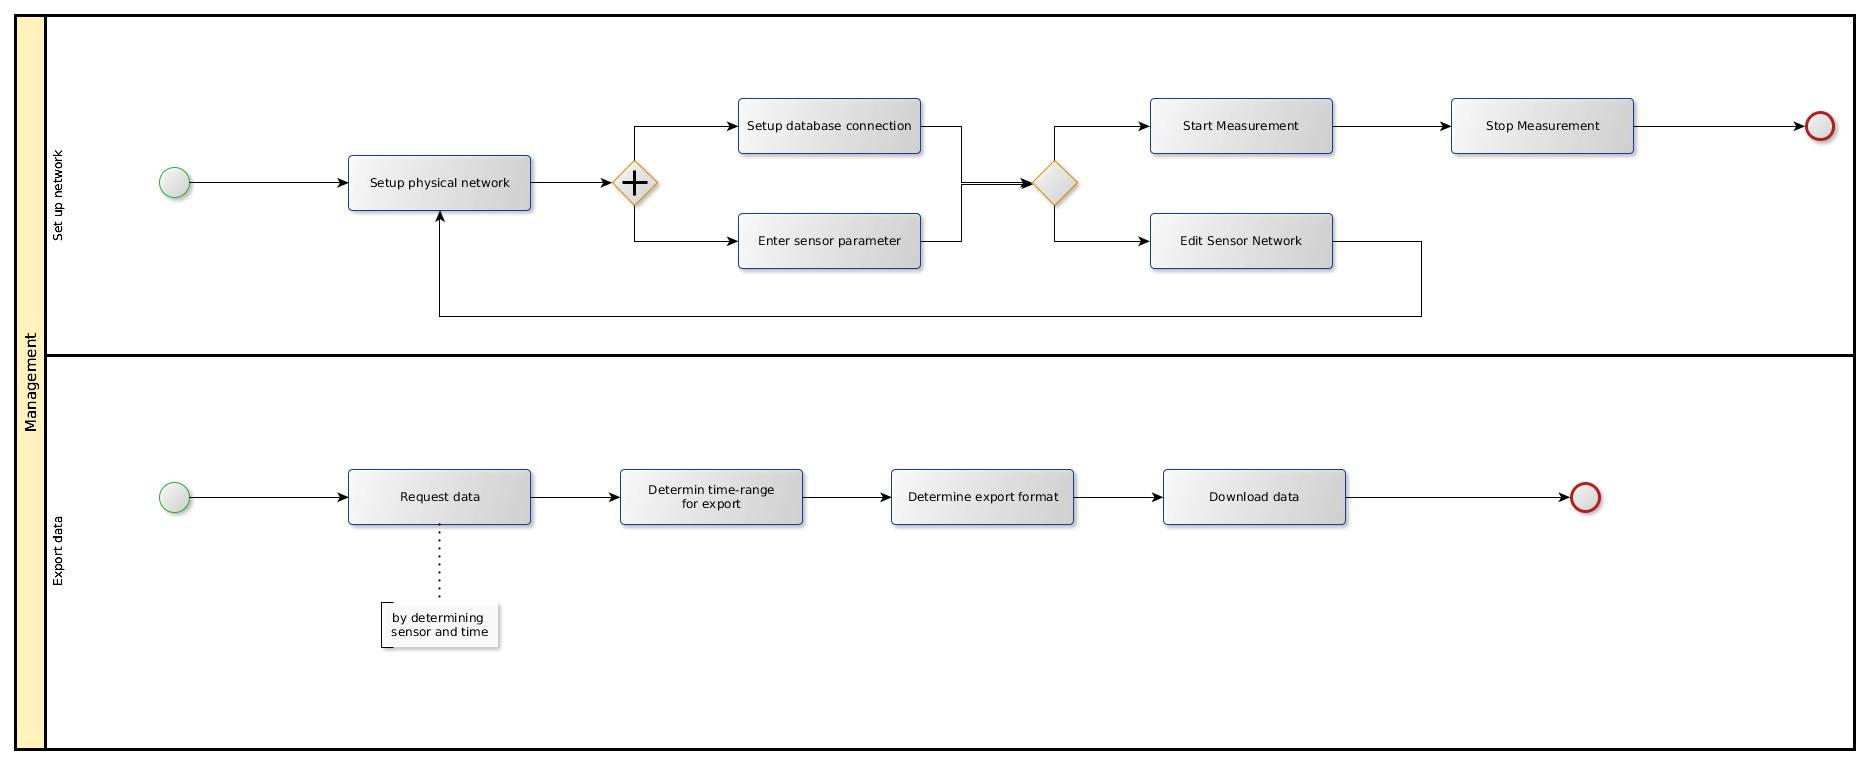
\includegraphics[scale=0.24]{graphics/bpmn_use-cases_management.jpg} 
	\caption{BPMN (Business Process Model and Notation) Model of the use cases describing central management proceedings. By F. H. Euteneuer 2013}
	 \label{fig:bpmn_use-case_management}
\end{figure}


\subsubsection{Measuring}

The measurement part might be the most important one within the system. This part is the only one which is describing a manual manipulation of the data in the database.

There are two identified use cases: The first is dealing with the initial data input which is the measurement see table \ref{table:use case description of "Measure data"}. In contrast to the automatic measurements, this is describing a discrete manual measurement, and the input of the data by hand.

And the second one is editing already existing data in the database see table \ref{table:use case description of "Edit data"}. This is a merely a standard operation for database related systems. Nevertheless, this task is related to the measurement task, in case of re-measuring data or validation of data.

\begin{table}[H]
\centering
\begin{tabular}{l | p{11cm}}
Name & Measure data\\ \hline 
Usergroup & Field engineer\\ \hline 
Goal & Input all data by hand  getting from standalone measurement device\\ \hline 
Precondition & Running system and access to database\\ \hline 
Postcondition & valid data in the database with full set of metadata\\ 
\end{tabular}
\caption{Use Cases tabular description of characteristics} 
\label{table:use case description of "Measure data"}
\end{table}

\begin{table}[H]
\centering
\begin{tabular}{l | p{11cm}}
Name & Edit data\\ \hline 
Usergroup & Office Engineer\\ \hline 
Goal & Specify data by parameter and input new values by hand or measurement\\ \hline 
Precondition & Running system and access to database\\ \hline 
Postcondition & changed data in the database with full set of metadata\\ 
\end{tabular}
\caption{Use Cases tabular description of characteristics} 
\label{table:use case description of "Edit data"}
\end{table}

When performing a manual measurement, most of the task described in the first line of the figure \ref{fig:bpmn_use-case_measuring} will be mandatory tasks. In the end the system will perform a quick analysis of the inserted data in order to validate the measurement. After this step the system will either point out possible errors, or it will approve the measurements, and write them into the database. The second line, the editing flow, is offering two options, one is a manual insert of new data, another would lead to a re-entering of the manual measurement flow, in order to overwrite the selected datasets with new measurements.

\begin{figure}[H]
	\centering
 	 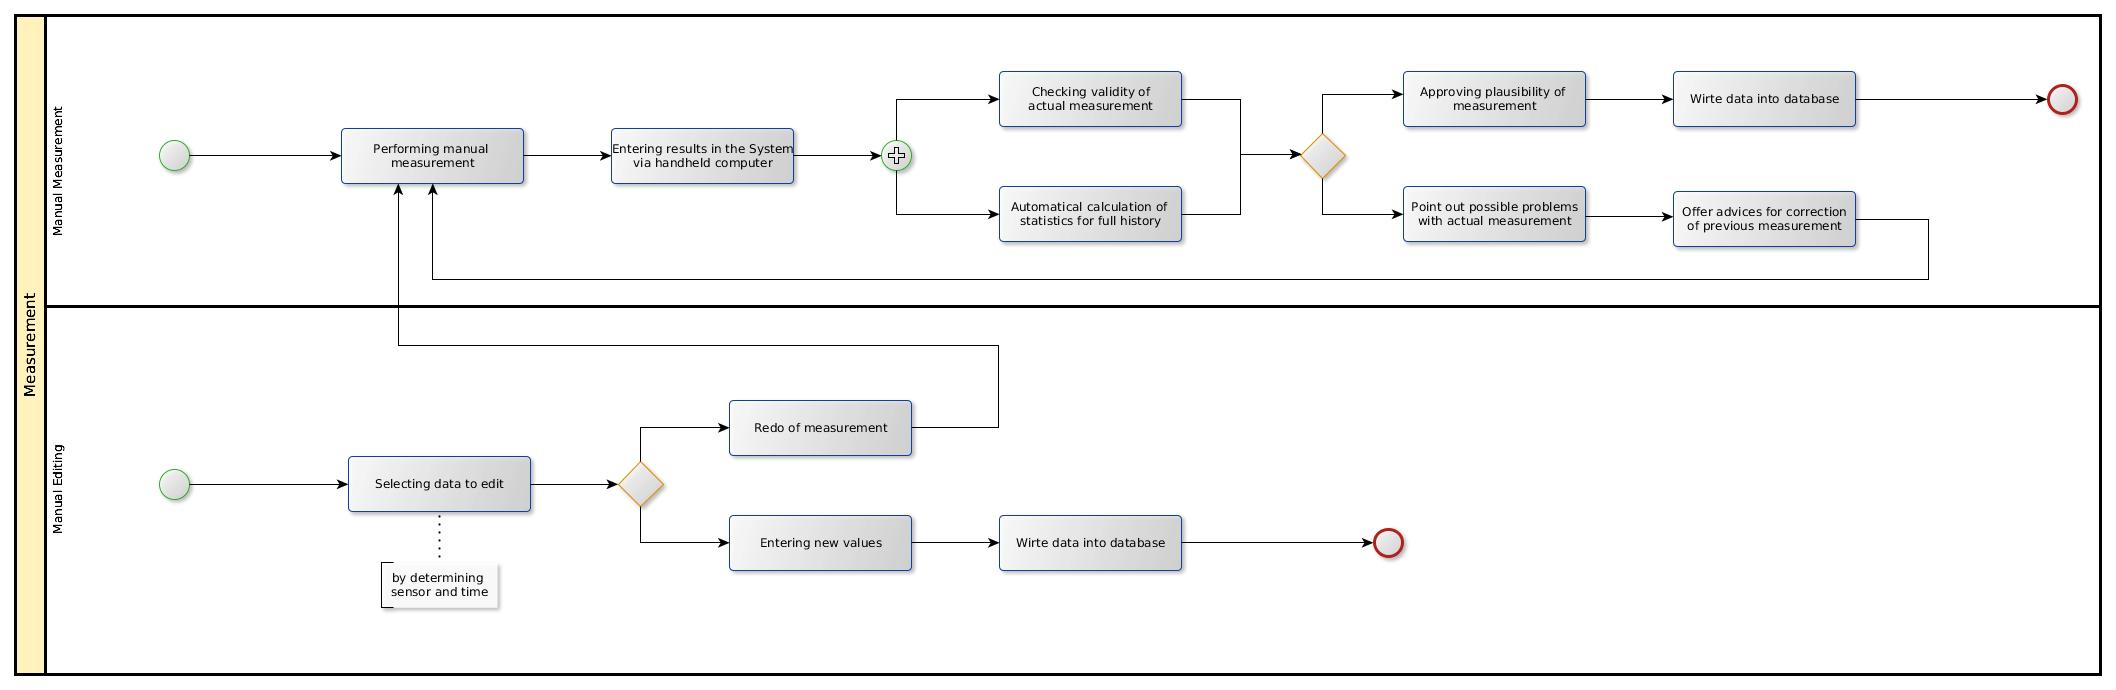
\includegraphics[scale=0.24]{graphics/bpmn_use-cases_measurement.jpg} 
	\caption{BPMN (Business Process Model and Notation) Model of the use cases describing central measuring proceedings. By F. H. Euteneuer 2013}
	 \label{fig:bpmn_use-case_measuring}
\end{figure}

\subsubsection{Analysis}

A complex part is the analysis functionalities of the system which will be described in this section. The analysis described here will be slightly different to the "ad hoc" statistics in the previous part which are leading to approved or discarded measurements. Those are checking the coherence of the performed measurements. The analysis described here are producing also easy and quick statistics, but in comparison to historical data see table \ref{table:use case description of "Analyse data"}. The user will be able to recheck if the measurements are leading to similar results, or if the measurements are possibly done with wrong parameters. 

The other analysis part is a visual analysis of the data (see table \ref{table:use case description "Visualise data"}). The system will here produce some graphics representing the measurement, the observed object and the related statistics. An optical validation of the performed measurements, and additionally to that, an optical representation of real-time data is a big advantage for the field-engineer (as described in the overall introduction).

\begin{table}[H]
\centering
\begin{tabular}{l | p{11cm}}
Name & Visualise data\\ \hline 
Usergroup & Field engineer\\ \hline 
Goal & Getting support by visualising measurements and interpretation\\ \hline 
Precondition & Existing meatadata for measurements\\ \hline 
Postcondition & meaningful and „supporting“ graphic\\
\end{tabular}
\caption{Use Cases tabular description of characteristics} 
\label{table:use case description "Visualise data"}
\end{table}

\begin{table}[H]
\centering
\begin{tabular}{l | p{11cm}}
Name & Analyse data\\ \hline 
Usergroup & Field engineer\\ \hline 
Goal & Getting information about validity of data in comparison to historical data\\ \hline 
Precondition & Amount of measurements higher then two\\ \hline 
Postcondition & information about validity of the data\\ 
\end{tabular}
\caption{Use Cases tabular description of characteristics} 
\label{table:use case description of "Analyse data"}
\end{table}

Figure \ref{fig:bpmn_use-case_analysis} is showing the two flows of the analysis part. The first line is describing the single steps of the analysis. For the analysis of data in context of historical data, the history has to be well defined. Therefore this is also part of the work-flow analysis.

The visualisation is divided into two different types of visualisations. The user can select a visualisation of the measured data. This might be represented by single geographic points. The type of visualisation is strongly depending on the type of the measurement instrument (e.g. an accelerometer is not changing its position, but it is changing the positions attributes). The second option is the visualisation of the statistics. Therefore the visualisation workflow is "calling" the function analysis in order to get the dataset specific statistics for its visualisation.

\begin{figure}[H]
	\centering
 	 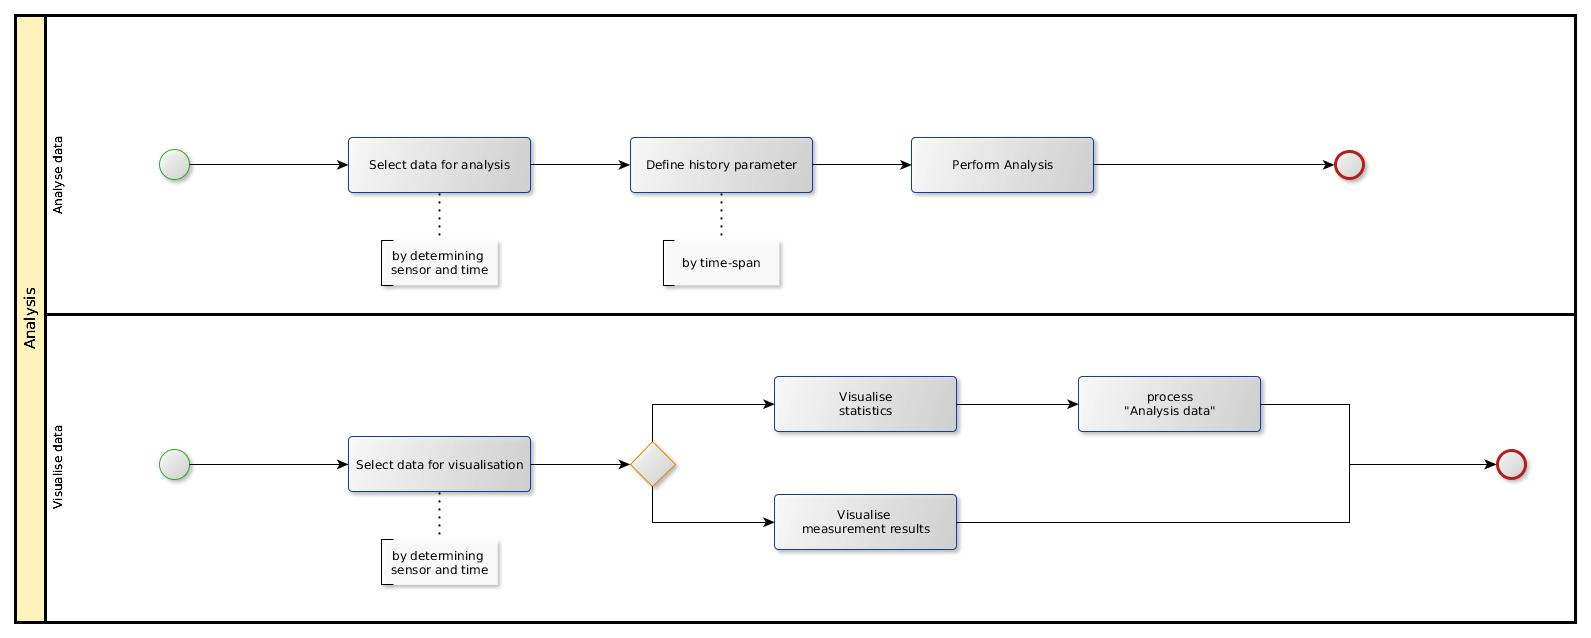
\includegraphics[scale=0.24]{graphics/bpmn_use-cases_analysis.jpg} 
	\caption{BPMN (Business Process Model and Notation) Model of the use cases describing central analysis proceedings. By F. H. Euteneuer 2013}
	 \label{fig:bpmn_use-case_analysis}
\end{figure}


\section{Product functionalities}
This part will describe the non-functional requirements of the system. This can be understood as a description of where the system will operate and how the software will operate. Non-functional requirements are requirements on a system which are not a technical functionality but a feature of the system.

The following list is describing those non-functional requirements:

\begin{description}
\item[portability] Since the system will be based on mobile devices, and those are not in any case running under windows, the software will be platform independent. Nevertheless also a web-based system is not possible, because the necessary internet connection will not be permanently available in field.
\item[performance] As described in the point before, the system will use different mobile platforms. Those do not have a hardware with a hight performance. Therefore the systems mobile part will be planed for a low performance.
\item[simplicity] The system will be used from field engineers which are working often under lots of negative influences of the environment. The system will be constructed as simply as possible to avoid unnecessary time costs for searching the right systems functionality.

\end{description}


\subsection{Fundamentals of Photovoltaik systems}

A Photovoltaic systems transduces solar radiation into electricity. The efficiency of a system depends on the properties of the used photovoltaic cells. Wagner (2010) \citen{Wagner2010} \\

\begin{figure}[hbt!]
\centering
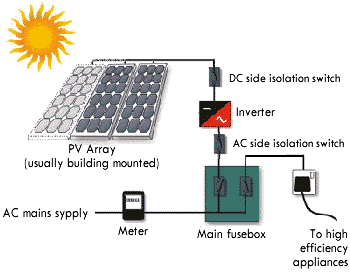
\includegraphics[width=0.7\textwidth]{phase2/group2/figure/pv-system-configuration.png}
\caption{Architecture of Photovaltaic system}
\label{fig:PV_system}
\end{figure}

The nominal power of a cell is given in Watt and often denoted as \(W_p\) (Watt Peak). It is acquired under standard test condition (STC an international standard) from the manufacturer of the photovoltaic cell. STC means, that the cell temperatur is \(25^\circ C\) and the irradiance is 1000 \(W/m^2\). The nominal power can be used to compare the power of photovoltiac cells of different manufactures. 
\\
The efficiency is given by the ratio between the produced energy and the energy radiated to the cell. It depends on the temperature of the photovoltaic cells. With increasing temperature the efficiency decreases. Often only one efficiency coefficient, including the efficiency of the power inverter, cable and accumulator, is given by the manufacturers.
\\
In addition a performance ratio is given most times. It is the ratio of the actual and the desired gain of the photovoltaic cell. It depends not only on the cell itself but also on the weather conditions, respectivly on the location. The desired gain is the efficiency of the installation under STC, assuming that the efficiency of the power inverter is \(100\%\). For a thin-layerd slicon cell, which is most common, the Performance ratio (PR) is \(84\% \) for Germany.
Wagner (2010)


\subsection{Fundamentals of Solar thermal systems}

Solar thermal collectors are devices, which transform radiation emitted by sun into heat. Basically, a collector consists of a box with a black glazed cover, containing a pipe, which uses all the space in the box. The radiation is adsorbed by the black glazing and heats up a fluid, such as water or oil, which runs through the pipe equipped in the  collector. The heated fluid can then be stored in insulated tanks, if it cannot be used directly.    In general solar collectors are used for use water in a household or for heating.\citen{Kalogirou}

basically, the efficiency of a solar thermal collector depends on the absorption of the glazing, the input fluid temperature , the average air temperature as well as the solar radiation of the region.
% global irradiance
\subsection{Global Irradiance}

The most important input value to calculate the Solar potential is the global radiation. The global radiation comprises the direct solar radiation and the diffuse radiation resulting from reflected or scattered sunlight. It depends on the location, the orientation of the roof surface and the inclination of the roof surface. The location is the latitude \(52^\circ 31' 45.0''\) and longitude \(13^\circ 19' 42.6''\)  of Moabit in Berlin. The orientation and the inclination are calculated from the CityGML Lod2 geometry. (European Database of Daylight and Solar Radiation)

\subsubsection{Orientation of the roof}

The azimuth angle \(\alpha\) represents the orientation of the roof. It is given by the angle between the normal vector of the roof \(n_r\) surface and the normal vector of xz plane \(n_{xz}\). 
\begin{eqnarray}
\label{eq:angle2vec}
\alpha = cos^{-1} ( \frac{\vec{n_r} \vec{n_{xz}}}{|n_r|  |n_{xz} | })
\end{eqnarray}

The direction of the normal vector is defined by the order of the point sequence forming the polygon ring of the roof surface. To calculate the orientation the positive normal vector is needed. If \(n_r\) has a negative z component \(n_r\) is converted to the positive normal vector. The calculated angle \(\alpha\) is always in a range between \(0^\circ-180^\circ\). Because the azimuth angle has a range of \(0^\circ-360^\circ\) we have to consider the sign of the x component of \(n_r\). Is the x component negative the azimuth angle is calculate with
\begin{eqnarray}
\alpha_o = 360^\circ - \alpha
\end{eqnarray}
else the azimuth angle \(\alpha_o\) is equal to \(\alpha\). 

\subsubsection{Inclination of the roof}
The inclination of the roof influences the input of solar radiation strongly and has to be considered. It is calculated as the angle between the normal vector of the roof surface \(n_r\) and the normal vector of the xy plane \(n_{xy}\). To calculate this angle equation \ref{eq:angle2vec} is used. Again the calculated angle ranges between \(0^\circ-180^\circ\), although the maximal tilt angle is \(90^\circ\). Therefore the tilt angle is
\begin{eqnarray}
t = 180^\circ - \alpha 
\end{eqnarray}
if \(\alpha > 90^\circ\) else \(t\) is equal \(\alpha\). For further calculation all roof surfaces with an inclination \(t<8^\circ\) are considered to be flat roofs and the angle \(t\) is set to \(0^\circ\).

\subsubsection{Satel-Light Database}
The estimation of the global irradiation for flat roof surfaces is simple, because no diffuse radiation effects the global radiation. For inclined surfaces the diffuse radiation resulting from reflected or scattered sunlight has to be considered. Because this is very complex we decided to use the European Database of Daylight and Solar Radiation (Satel-Light), which provides for every location within Europe the global radiation on tilted else well as flat roof surfaces with arbitrary orientation. We created a LookUp table for Berlin, which contains the global radiation for the inclination in \(10^\circ\) degree steps and the orientation in \(45^\circ\) steps. The resulting table is shown in figure \ref{fig:rad_table}.

\begin{figure}[hbt!]
\centering
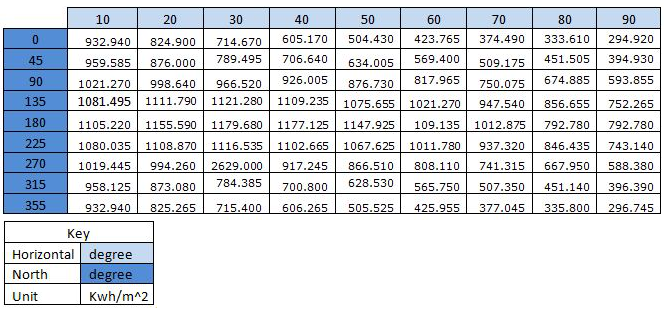
\includegraphics[width=0.9\textwidth]{phase2/group2/figure/table_global_radiation.png}
\caption{LookUp table for the global radiation for Berlin}
\label{fig:rad_table}
\end{figure}

\subsection{Reduction of Roof Surface Area due to Roof Equipment}
\label{sec:roofarea}
The main problem when using a LOD 2 model is that the suitable roof area is not known. Fact is, that not 100\% of the roof can be used to install solar panels, since roofs may have dormers, antennas or chimneys which are not part of the LOD2 model. But the roof equipment is considered for the Solar Atlas Berlin and with use of this data source empirical reduction factors may be computed. Therefore group 2 implemented a program, which reads a cityGML file, containing all buildings of the test area (~1000 buildings) and computes the reduction factor as in Equation \ref{eq:roof}.

\begin{align}
\label{eq:roof}
r_E &= \frac{A_{SAB}}{A_{LOD2}} \\\notag\\\notag
\text{with:}&\\\notag
r_E &:\text{ empirical reduction factor}\\\notag
A_{SAB} &: \text{Roof Area according to solar atlas Berlin }\\\notag
A_{LOD2} &: \text{ roof area calculated from LOD2 model in 3D CityDB }\\\notag
\end{align}

The Solar Atlas Berlin provides different areas for photovoltaic and solar thermal systems. Therefore also different reduction factors are computed. The reduction factors are also separated between exclusively flat roof and mixed roofs, contain flat as well as tilted surfaces. This is important because flat roofs are more likely equipped. Additionally, the age class of the building has been taken into account. Tables \ref{tab:roofarea_st} and \ref{tab:roofarea_pv} show the result, including the number of surface and the variance of the value. It can be seen that, some reduction factors are not representative, because not enough roofs of this type are in the test area. With the use of a database of entire Berlin might fix the Problem.

 

\begin{table}
\centering 

\begin{tabular}{|c||c|c|c||c|c|c|}
  \hline
  \multirow{2}{*}{Age Class} & \multicolumn{3}{|c||}{flat roof} &  \multicolumn{3}{|c|}{mixed roof}\\
  \cline{2-7}
  & $r_E$ & count & $\sigma^2$  & $r_E$ & count & $\sigma^2$\\
  \hline
1899&0.198&94&0.016&0.440&199&0.056\\\hline
1918&0.152&56&0.019&0.435&233&0.059\\\hline
1932&0.167&13&0.017&0.506&9&0.048\\\hline
1945&0.304&2&0.0008&0.765&1&0.000\\\hline
1961&0.221&74&0.013&0.581&56&0.049\\\hline
1974&0.198&90&0.015&0.371&17&0.080\\\hline
1993&0.219&66&0.006&0.293&5&0.016\\\hline
2012&0.149&91&0.019&0.487&21&0.165\\\hline
\end{tabular}
\caption{empirical reduction factors for calculation of energy gain using solar thermal collectors }
 \label{tab:roofarea_st}
\end{table}

\begin{table}
\centering 
\begin{tabular}{|c||c|c|c||c|c|c|}
  \hline
  \multirow{2}{*}{Age Class} & \multicolumn{3}{|c||}{flat roof} &  \multicolumn{3}{|c|}{mixed roof}\\
  \cline{2-7}
  & $r_E$ & count & $\sigma^2$  & $r_E$ & count & $\sigma^2$\\
  \hline
1899&0.127&94&0.019&0.349&199&0.050\\\hline
1918&0.097&56&0.016&0.323&233&0.053\\\hline
1932&0.056&13&0.008&0.403&9&0.076\\\hline
1945&0.000&2&0.000&0.730&1&0.000\\\hline
1961&0.147&74&0.015&0.498&56&0.050\\\hline
1974&0.129&90&0.016&0.289&17&0.081\\\hline
1993&0.128&66&0.011&0.146&5&0.013\\\hline
2012&0.090&91&0.016&0.399&21&0.147\\\hline
\end{tabular}
\caption{empirical reduction factors for calculation of energy gain using photovoltaic modules }
 \label{tab:roofarea_pv}
\end{table}


\subsection{Shadowing}
\label{sec:shadowing}
Roof surfaces may be shadowed by several object, such as other buildings, trees or even equipment on the roof itself. Since, the data source is a LOD 2 model only other buildings can be considered, because trees and roof equipment are not part of the model. The consideration of the shadowing may be done with a complicated illumination computation. Since this project is limited in time this is not possible. Therefore only a simple approach is applied, which completely ignore buildings which are shadowed, rather then adjusting the daily global irradiance on the specific surface.
Within the simple approach a building is neglected, if there is a neighboured building which is $x$ higher and is within a certain radius $r$. Only buildings between an azimuth of 90° to 270° are taken into account, as shown in Figure \ref{fig:shadow}.

\begin{figure}[ht]
	\centering
	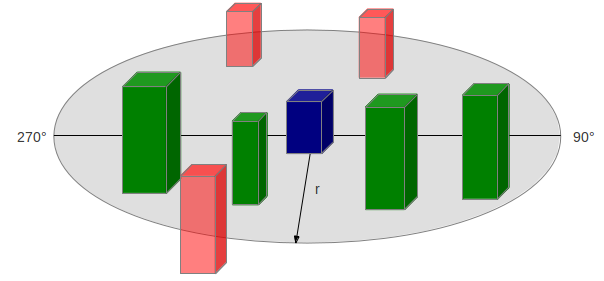
\includegraphics[width=0.7\textwidth]{phase2/group2/figure/fig_shadow.png}
	\caption{The green buildings are candidates, which may shadow the blue building}
	\label{fig:shadow}
\end{figure}

The implemented algorithm starts with iterating over all buildings and storing them in a spatial tree to make them easy queryable. After that before a potential of a building is calculated it will be checked if there are candidate buildings which are within the radius $r$. The list of candidates is checked for buildings which also meet the other conditions, such as an azimuth between $90^\circ$ and $270^\circ$ and if the building is $x$ times higher. If both conditions are met, the building will be neglected for the potential calculation. 
\subsection{Calculation of the potential}

The calculation begins with the reduction of the roof area according to the building age class as described in chapter \ref{sec:roofarea}. If the roof surface is a flat roof ($tilt < 8 ^\circ$) the modules cannot directly mounted of the roof surface. To bring the modules in an optimal tilt angle they are mounted on a mounting system of the roof. Because they are tilted they might shadow the neighboring modules, therefore a certain distance between the modules is necessary as shown in Figure \ref{fig:flatroof}. The distance has to be $c=2.75$ times longer then the width of the ground of the module $w$.
%TODO: ADD REFERENCE!
\begin{figure}[ht]
	\centering
	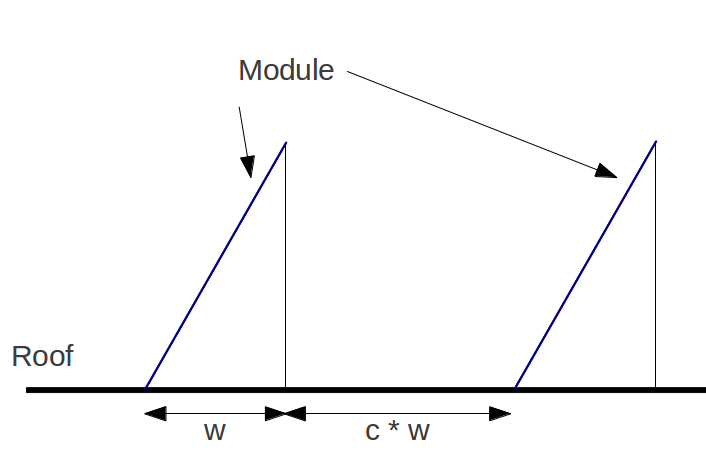
\includegraphics[width=0.5\textwidth]{phase2/group2/figure/flatroofreduction.png}
	\caption{Solar Modules mounted on a mounting system of a flat roof}
	\label{fig:flatroof}
\end{figure}
Furthermore the global irradiance has to be picked from the look-up table. According to Solar Atlas Berlin \citen{solaratlas} areas with a global irradiance less than $905 Wh/m^2$ have to be neglected. Also surface are neglected which have a smaller area then $5m^2$. It is assumed that it is economically not worth the mount modules on such a small roof. The actual calculation of the potential highly depends on the type of module. This will be explained in the following sub sections.



\subsubsection{Potential of Photovoltiac systems}
To calculate the potential of photovoltiac systems two approaches were applied. First the estimation as described by Wagner (2010) \citen{Wagner2010} was implemented. According to Wagner (2010) the energy gain of a photovoltiac system can be calculated with 

\begin{align}
\label{eq:pv_calc}
E &= M \cdot GA \cdot \frac{P}{E_0} \cdot PR \cdot \eta_{EUR} \cdot \eta_l \\\notag\\\notag
\text{with:}&\\\notag
E &:\text{total energy gain per year \(kWh/a\)} \\\notag
E_0 &:\text{1000 \(W/m^2\)} \\\notag
M &:\text{Number of Modules} \\\notag
PR &:\text {Performance ratio} \\\notag
P &:\text{nominal power \(W\)} \\\notag
\eta_{EUR} &:\text{euro inverter efficiency} \\\notag
\eta_l&:\text{transmission efficiency} \\\notag
GA &:\text{Global Irradiation \(kWh/m^2 a\)} \notag
\end{align}

The parameters \(P\),\(\eta_{EUR}\),\(\eta_l\) and \(M\)depend on the photovoltaic cell and the inverter. Values for these parameters are taken from real photovoltiac cells. For the calculations the silicon cell BP 585F from BP Solar \citen{BPSolar} combined with the inverter SP 2500-450 from the company Sun Power \citen{SunPower} has been used. The inverter efficiency is \(\eta_{EUR} = 15 \%\) and the transmission efficiency is set to \(\eta_l = 9\%\). The nominal power of the cell is \(P_0 = 85 W\). This calculation method allows to use real data of photovoltiac cells and considers the inverter.
\\

Because the the Solar Atlas Berlin is the only available reference, finally a second approach according to the Solar Atlas was used. The calculation of the photovoltiac energy is simplified and finally done with equation \ref{eq:pv_calc_SAB}. Where the efficiency coefficient is set to \(e=15\%\) and the system area is the reduced roof surface area.

\begin{align}
\label{eq:pv_calc_SAB}
E &= A \cdot GA \cdot PR \cdot e \\\notag\\\notag
\text{with:}&\\\notag
E &:\text{total energy gain per year \(kWh/a\)} \\\notag
A &:\text{System Area \(m^2\)} \\\notag
e &:\text{efficiency coefficient} \\\notag
GA &:\text{Global Irradiation \(kWh/m^2 a\)} \notag
\end{align}





\subsubsection{Solar Thermal}
The calculation of the potential of solar thermal modules was done as described in Struckmann (2008) \citen{struckmann2008}. According to Struckmann (2008) the useful energy gain $Q_U$ of a solar thermal module is calculated with the formula shown in Equation \ref{eq:st_calc}. Figure \ref{fig:st_module} shows a sketch of a typical solar thermal module and shows the parameter, which are necessary to compute $Q_U$  

\begin{align}
\label{eq:st_calc}
Q_U &= F_R  A \left( I \tau \alpha - U_L \left(T_i - T_a \right) \right)\\\notag\\\notag
\text{with:}&\\\notag
F_R &:\text{ Efficiency Coefficient of the module}\\\notag
A &: \text{ module area, $m^2$}\\\notag
I &: \text{ Solar radiation, $W/m^2$ }\\\notag
\tau &: \text{ transmission coefficient of glazing}\\\notag
\alpha &: \text{ absorption coefficient of plate}\\\notag
U_L &: \text{ collector overall heat loss coefficient, $W/m^2$}\\\notag
T_i &: \text{ input fluid temperature, $^\circ C$}\\\notag
T_a &: \text{ average outside air temperature, $^\circ C$}\notag
\end{align}

\begin{figure}[ht]
	\centering
	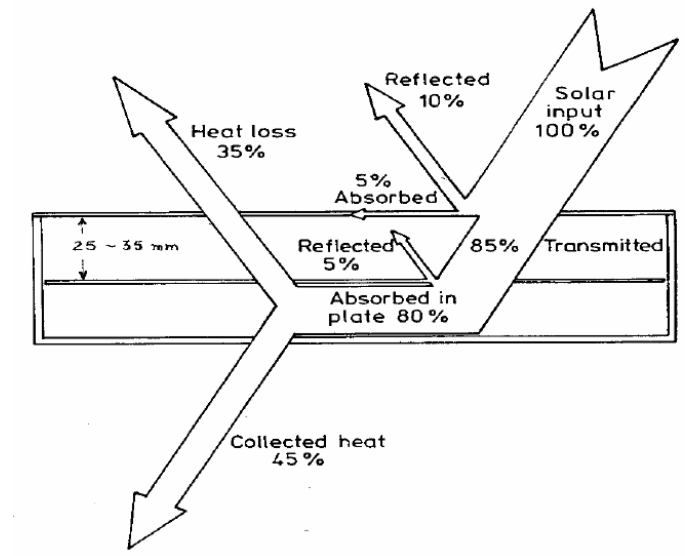
\includegraphics[width=0.5\textwidth]{phase2/group2/figure/st_module.png}
	\caption{typical module with visualization of calculation parameters (Struckmann (2008))}
	\label{fig:st_module}
\end{figure}

For the calculation of the potential a standard solar thermal module has been taken, the TitanPower-AL2DH Flat Plate Collector from the company SunMaxxSolar \citen{sunmaxx}. The efficiency coefficient is assumed to be $F_R = 0.35$ since this value is also used by SimuPLAN for Solar Atlas Berlin. The input fluid temperature is assumed to be $T_i = 10 ^\circ C$ which seems to be a realistic value for the region of Berlin.  Also the average outside air temperature is taken as  $T_a = 10 ^\circ C$.



\subsection{Validation of Result}
The results are compared and validated against the values computed for the project "Solar Atlas Berlin". According to the roof area which is suitable for solar panels per building, the geometry data source of the Solar Atlas is expected to be of higher quality, because the data has been acquired using a laser scanning system. Therefore, the usable roof area may be exactly predicted for each building. Usable roof area is the area which is not used for any equipment on the roof, such as dormer, chimneys or antennas. The data source used within the GIS Project is an LOD2 Model of Berlin, which does not contain information about roof equipment. For this reason, we use the Solar Atlas Berlin to validate our results.

The value which is validated is calculated potential in MWh/a for photovoltaic systems as well as solar thermal systems. For each building in the test area the difference between the potential given from Solar Atlas Berlin and the potential calculate within the project in calculated. Note, that photovoltaic and solar thermal system are always considered separately.

Out of the differences, the standard deviation can be computed. Since the expectation is known ($e=0$, no difference) the standard deviation is computed as in Equation \ref{eq:validation}.

\begin{align}
\label{eq:validation}
\sigma = \sqrt{\frac{1}{n} \sum\limits_{i=1}^n (diff_i - e )^2}
\end{align}

For the test area a standard deviation of $\sigma_{pv} = 6.45 Mwh/a$ for photovoltaic and $\sigma_{st} = 10.49 Mwh/a$ for solar thermal systems has been reached. A weak spot of this approach is, that outliers influence the result. Although most of the differences are close to zero, the standard deviation is relatively high.
\subsection{Visualization}

To visualize the results a new appearance theme is added using citygml4j. To do this the results have to be classified. For both photovoltaic and solar thermal potential three classes are defined.
\\
Photovoltaic
\begin{itemize}
\item Photovoltaic potential classes
\subitem \(>=50kWh/m^2a\), very good, color: red
\subitem \(<50kWh/m^2a\), good, color: orange
\subitem \(<30kWh/m^2a\), limited, color: yellow
\item Solar thermal potential classes
\subitem \(>=100kWh/m^2a\), very good, color: red
\subitem \(<100kWh/m^2a\), good, color: orange
\subitem \(<50kWh/m^2a\), limited, color: yellow
\end{itemize}

Due to time problems the classification is not optimal. The class boundaries are only empirical values. Furthermore the total energy output depends on the roof area. Which leads to a classification of small roofs to low class although the orientation optimal and the global radiation high. For further investigations this classification should be optimized. The Solar Atlas Berlin uses total global radiation to classify the potential, which could be used as better model.
The new appearance theme is created with citygml4j. Each roof surfaces is added as appearance member. According to the class the are linked with the corresponding diffuse color.
After writing the new CityGML file with all energy related attributes and the new appearance theme. The file is imported to a empty database. Subsequently a KML/Collada export is used to export a KML file with the new appearance IGG\_PV\_Potential. Additionally the address and the values of photovoltaic and solar thermal potential are stored in KML balloons for each building. Figure \ref{fig:vis} shows the resulting KML of the statistical block in Google Earth.

\begin{figure}[hbt!]
\centering
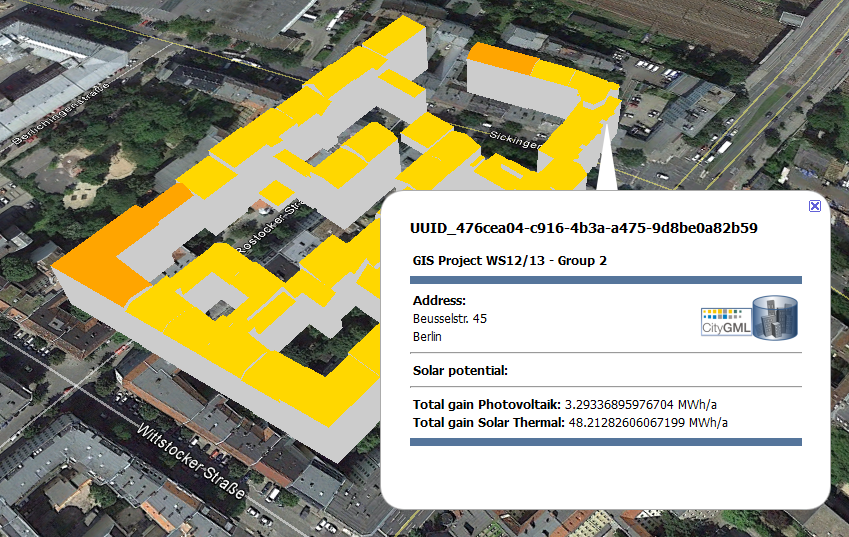
\includegraphics[width=0.7\textwidth]{phase2/group2/figure/viz.png}
\caption{KML export}
\label{fig:vis}
\end{figure}

\subsection{Conclusion}
% TODO: point out weak spots of our implementation and validation (e.g. Solar Atlas is not reliable enough, roof surfaces are not merged)
It can be concluded that the estimation of the photovoltaic potential as well as the solar thermal potential is only applicable to a limited extend. For single buildings the estimation is far to inaccurate, whereas the results for a statistical block become more reliable. The standard deviation for both potentials is too high, it is close to the mean of the potential, which means the result is for a high percentage of all buildings is totally wrong. But the standard deviation is calculated on the basis of the values given by the Solar Atlas Berlin. Therefore the values of the Solar Atlas Berlin are assumed to be correct. That this is not always the case was proved at least with on building. The potential was shifted by one decimal place. Also the geometry data is not sufficient. The used Lod2 (Level of detail 2) geometry only comprises simple polygons to describe the roof surfaces. No geometry of additional roof structures, as dormers, antennas or chimneys are  available. Furthermore the roof surfaces 
representing one roof within the 3D City DB does not always correspond to the real roof surfaces. Some roof surfaces are represented by several small surfaces in the Database. This leads to errors for the estimation of the potentials, because horizontal roof surfaces smaller \(40m^2\) and tilted roof surfaces smaller \(15m^2\) are ignored during the calculation of the potential. \\
The solar potential of roofs depends strongly on the input of solar radiation, which in turn is strongly influenced by shadows. The used shadowing model is very simple. Only shadows due to very high neighboring buildings are considered. Shadows due to additional roof construction are neglected. Tests showed that only a few buildings were neglected due to the implemented shadow model. \\
Nevertheless the estimation of solar potential with existing CityGML data can be very fast and cheap, because no expansive Lidar data is necessary.\\
For the current implementation the disadvantages outbalance the advantages. The results are not accurate enough to use this approach 
\subsection{Future Work}
%TODO: things which may be implemented to improve the results. describe possible solutions to fix the  ``weak spots'' which we pointed %out in the conclusion.

Further investigations to improve the calculation model can lead to better results. Instead of an Lod 2 geometry a higher level of detail as Lod 3 can be used, which describes the geometry of the roofs in more detail. To avoid the neglection of too small roof surfaces due to wrong surface separations, neighboring roof surfaces with equal inclination and orientation should be merged in future.\\
In addition a high order shadow model, which considers partly shadowing of a roof surfaces due to other buildings and shadowing due to additional roof structures. Until now the shadow model is not capable of reducing the global irradiation, but neglects the whole building. The new model should be able to deal with this reduction due to partly shadowed roof surfaces.

%\end{document}
